\subsubsection{WW production}
\label{sss-WWprod}

%short intro
The \WW\ production process has the highest production cross section
among the massive vector di-boson processes. It is also an important
background process to Higgs production and to searches for new physics.
%analysis CMS and ATLAS.
%    ** ATLAS (5.6ifb, 7TeV, TGC), Phys. Rev. D 87, 112001 (2013), http://arxiv.org/abs/1210.2979
%	    ATLAS (20ifb 8TeV), https://atlas.web.cern.ch/Atlas/GROUPS/PHYSICS/CONFNOTES/ATLAS-CONF-2014-033/ 
%    ** CMS (7 TeV, 5 fb-1, TGC)  WW cross section in the lvlv channel at 7 TeV  http://arxiv.org/abs/1306.1126
%    ** CMS (8 TeV, 3.5 fb-1 WW, 5.3 fb-1 ZZ) , Phys. Lett. B 721 (2013) 190, WW and ZZ at 8 TeV, http://arxiv.org/abs/1301.4698 
%	    CMS (20ifb, 8TeV), submitted to EPJC,  http://arxiv.org/abs/1507.03268
ATLAS and CMS, observed the \WW\ production process in 
the fully leptonic channel and published results for 7 TeV 
(ATLAS~\cite{ATLAS:2012mec}, CMS~\cite{Chatrchyan:2013yaa}) and
8 TeV (CMS~\cite{Chatrchyan:2013oev}) center-of-mass energy. 
%decay channels
Three final states, namely $ee$, $\mu\mu$, and $e\mu$ are included in the analyses. 
The contribution from leptonically decaying $\tau$ leptons is included in the signal
definition. Although the production cross section is relatively high, the signature of two opposite 
sign leptons and missing transverse energy is shared with many processes and a careful
control of the backgrounds is necessary to achieve a precise measurement.

%Theoretical calculations
% TBD -> General section about theoretical calculations?

%Selections
Candidate $\WW$ events are selected by requiring two oppositely-charged leptons 
accompanied with large \MET. 
%Backgrounds
The dominant background sources are \ttbar\; and single top quark, 
$\W/$+jets, followed by $\Zzero/\gamma^{*}$+jets production.
To suppress the dominant \ttbar\; background, events with one or more jets are rejected.   
Additional requirements on \MET\ and the use of top quark taggers further reduce the residual background
%ATLAS: 685 WW, 275 background => b / (s+b) = 29%
%CMS: 824WW, 369 background => b / (s+b) = 31%
to about 30\%.  
%systematics
The dominant systematic uncertainty is related to the jet veto efficiency 
and estimated to be about 5\% for the \WW\, production. 
The experiments quote a theoretical uncertainty on the signal acceptance due to 
variations of the parton distribution functions and renormalization and factorization 
scales in the range of 1-2\%.

% Results at the end
% total xsec
% ATLAS 7TeV 4.6 ifb: xsec(WW) = 51.9 +- 2.0 (stat) +- 3.9 (sys) +- 2.0 (lum) pb
%                     xsec_theo(WW) = 44.7 +2.1 -1.9 pb
% CMS 7TeV 4.9 ifb: xsec(ww) = 52.4 +- 2.0 (stat) +- 4.5 (syst) +- 1.2 (lum) pb
%                   xsec_theo(WW) = 47.0 +- 2.0 pb
% CMS 8TeV 5ifb: xsec(WW) = 69.9 +- 2.8 (stat) +- 5.6 (sys) +- 3.1 (lum) pb
%                xsec_theo(WW) = 57.3 +2.3 -1.6 pb (not including H ~ 4%)

% definition of total xsecs might differ (inclusion of higgs or not).
Both ATLAS and CMS provide a measurement of the total cross section for the process $pp \rightarrow \WW$
and compare to theoretical calculations. The Higgs process contributes with about 4\% to the total 
cross section and has not been taken into account in the comparison to the SM predictions.
The total cross section results are summarized in Table~\ref{tab:sss-WWprod-xsec}.
A good agreement between the experiments for the measured cross section as well as for the theoretical predictions
is observed.
% fiducial xsec
A normalized differential measurement of the fiducial cross section in bins of $\pt$ of the leading lepton is presented by ATLAS,
as shown in Figure~\ref{fig:sss-WWprod-pt-fiducial}. The unfolded spectrum is in agreement with the SM prediction.

\begin{table}[htp]

\begin{center}
\resizebox{\textwidth}{!}{
\begin{tabular}{|c|c|c|c|c|c|}
Experiment & cross section & \rts\; [TeV] & measured [pb]  & predicted [pb] & reference  \\ \hline
ATLAS & total & 7 & {51.9 $\pm 2.0$  (stat.) $\pm$ ${3.9}$ (syst.) $\pm$ 2.0 (lumi.) }  & {44.7 $^{+2.1}_{-1.9}$ } & \cite{ATLAS:2012mec} \\
CMS & total & 7 & {52.4 $\pm 2.0$  (stat.) $\pm$ ${4.5}$ (syst.) $\pm$ 1.2 (lumi.) }  & {47.0 $\pm 2.0$ } & \cite{Chatrchyan:2013yaa} \\
CMS & total & 8 & {69.9 $\pm 2.8$  (stat.) $\pm$ ${5.6}$ (syst.) $\pm$ 3.1 (lumi.) }  & {57.3 $^{+2.3}_{-1.6}$} & \cite{Chatrchyan:2013yaa} \\
\end{tabular}
}
\caption{Summary of measured fiducial and total $\WW$ production cross sections from ATLAS and CMS 
at 7 and 8 TeV center-of-mass energies in the $\lnu\lnu$ final state. The prediction are calculated at NLO in $\alpha_s$.}
\end{center}
\label{tab:sss-WWprod-xsec}
\end{table}%

% unfolded spectra
% https://atlas.web.cern.ch/Atlas/GROUPS/PHYSICS/PAPERS/STDM-2012-01/fig_07.pdf
% 
\begin{figure}[htbp]
  \begin{center}
  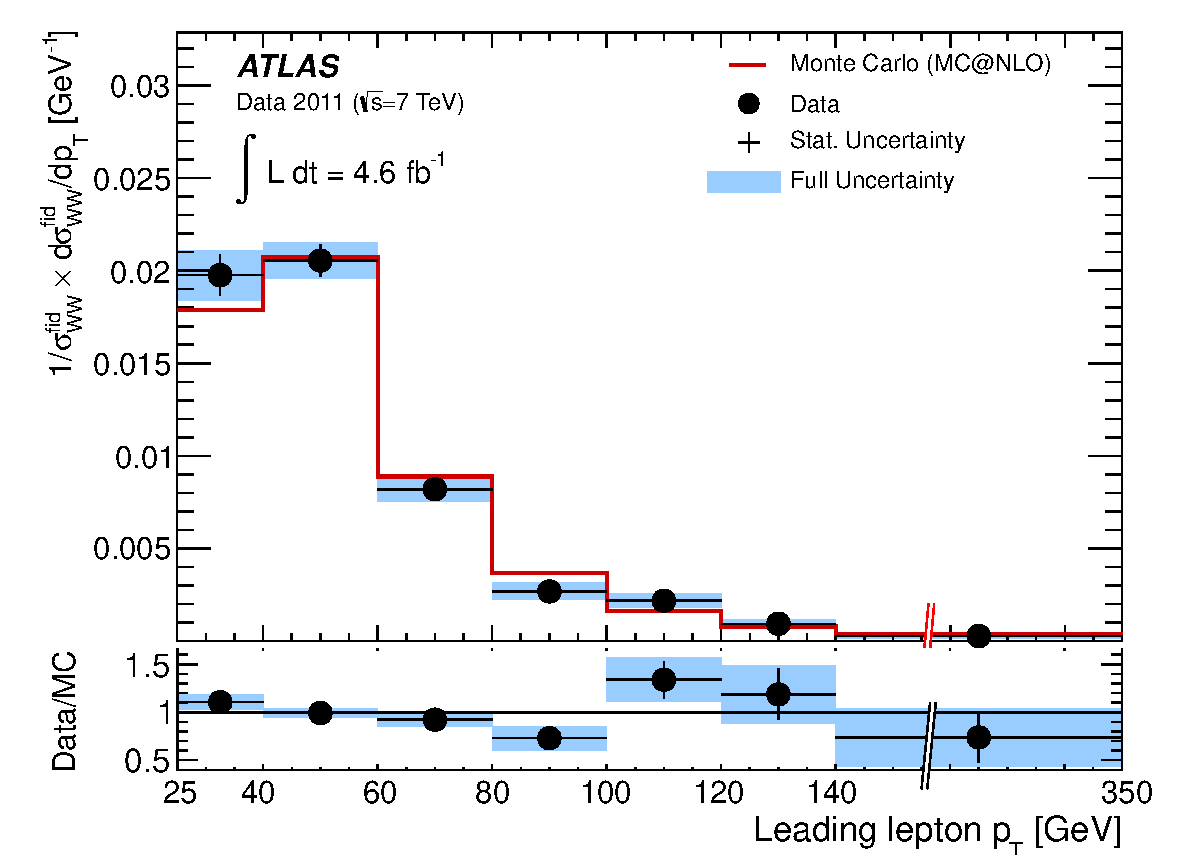
\includegraphics[width=0.45\textwidth]{figures/sss-inclboson-diboson-wwprod-pt-fiducial.pdf}
  \caption{ATLAS measurement~\cite{ATLAS:2012mec} of the transverse momentum of the leading lepton in \WW events compared with the SM prediction at $\rts = 7\TeV$. The full uncertainty contains statistical and systematic uncertainties.}
\label{fig:sss-WWprod-pt-fiducial}
\end{center}
\end{figure}


%%%%
% THIS MIGHT GO INTO THE SECTION ON TGC
% aTGC
The leading lepton $\pt$ spectrum of the \WW process is sensitive to anomalous gauge boson coupling parameters
\dkg,  \dkz, \lg, \lz, and \dgz. Both ATLAS and CMS quote limits in the LEP 
parametrization~\cite{Gounaris:1996rz} that introduces $SU(2) \times U(1)$ gauge invariance 
constraints to reduce the number of free parameters to \dgz,  \dkg, and \lz. The obtained limits assuming 
no form factor are compared for both expected and measured 95\% CL limits in Table~\ref{tab:sss-WZprod-ATGC}.

\begin{table}\centering
\begin{tabular}{cccc}
\hline
& Observed (CMS) & Observed (ATLAS) & Expected (ATLAS)\\
\hline
$\dgz$ & $[-0.095, 0.095]$ & $[-0.039, 0.052]$ & $[-0.039, 0.052]$ \\
$\dkg$ & $[-0.21, 0.22]$ & $[-0.14, 0.14 ]$ & $[-0.13, 0.13]$ \\
% ATLAS DKZ limits converted to DKG with DKG = c2/s2(DG1-DKZ) = 3.3252 * (-DKZ) [DG1 == 0]
$\lz$ & $[-0.048, 0.048]$ & $[-0.062, 0.059]$ & $[-0.060, 0.059]$ \\
\hline
\end{tabular}
\caption{Expected and observed 95\% CL limits on the ATGC parameters 
\dkg, \lz\ and \dgz\; in the LEP parametrization derived from the leading lepton $\pt$ spectrum in \WW production at 7 TeV (ATLAS~\cite{ATLAS:2012mec}, CMS~\cite{Chatrchyan:2013yaa}). No form-factor is applied to the ATGC parameters.}
\label{tab:sss-WZprod-ATGC}
\end{table}





